\documentclass{article}

\usepackage[final]{neurips_2025}
\makeatletter\renewcommand{\@neuripsyear}{2026}\makeatother

\usepackage[utf8]{inputenc}
\usepackage[T1]{fontenc}
\usepackage{lmodern}
\usepackage{hyperref}
\usepackage{url}
\usepackage{booktabs}
\usepackage{amsfonts}
\usepackage{amsmath}
\usepackage{amssymb}
\usepackage{nicefrac}
\usepackage{microtype}
\usepackage{xcolor}
\usepackage{colortbl}
\usepackage{graphicx}
\usepackage{subcaption}
\usepackage{multirow}
\usepackage{algorithm}
\usepackage{algorithmic}
\usepackage{tablefootnote}
\usepackage{enumitem}

\definecolor{improve}{RGB}{0,128,0}
\definecolor{decline}{RGB}{200,0,0}
\newcommand{\up}[1]{\textcolor{improve}{\textbf{+#1}}}
\newcommand{\down}[1]{\textcolor{decline}{\textbf{#1}}}
\newcommand{\ci}[2]{\scriptsize[#1,\,#2]}
\DeclareMathOperator*{\argmax}{arg\,max}
\DeclareMathOperator*{\argmin}{arg\,min}
\newcommand{\adathink}{\textsc{AdaThink}}

% NeurIPS checklist answer macros (only define if not already in .sty)
\providecommand{\answerYes}[1]{\textbf{Yes.} #1}
\providecommand{\answerNo}[1]{\textbf{No.} #1}
\providecommand{\answerNA}[1]{\textbf{N/A.} #1}

\title{\adathink{}: Adaptive Budget Allocation for\\Test-Time Compute in Large Language Models}

\author{
  Anonymous Author(s)
}

\begin{document}

\maketitle

\begin{abstract}
Scaling test-time compute via extended chain-of-thought reasoning improves LLM accuracy on hard problems, but we show that this improvement is far from uniform: fixed budgets \emph{systematically overthink easy questions and undercompute hard ones}, creating structured heterogeneity that simple post-hoc controllers can exploit.
We introduce \adathink{}, a training-free, inference-only framework that allocates per-question reasoning tokens based on difficulty signals extracted from a single low-budget probe pass---requiring no model modification or fine-tuning.
Our primary controller is a lookup table over three binary features (answer presence, token utilization, answer consistency) optimized via leave-one-subset-out cross-validation.
Despite its simplicity, this 3-bit template closes $76\%$ of the gap to an oracle budget selector on GSM8K-27B.
Evaluated across three benchmarks (GSM8K, MATH500, BIG-Bench Hard) and two Qwen model scales (8B and 27B), the template controller achieves \textbf{+11.3--28.9}\,pp accuracy gains over matched fixed-budget baselines, with all CIs excluding zero.
The two-pass overhead is offset by accuracy improvements, yielding positive utility gains ($+7.4$--$23.1$\,pp) across all settings.
Feature-stratified analysis reveals the mechanism: $\sim$13\% of questions are ``easy'' (60\% overthinking rate at the max budget), while $\sim$60\% are ``hard'' and benefit from budget escalation.
Cross-benchmark transfer shows the difficulty pattern generalizes: templates learned on MATH500 transfer perfectly to BBH.
\end{abstract}

\section{Introduction}
\label{sec:intro}

Large language models (LLMs) increasingly rely on extended chain-of-thought (CoT) reasoning at inference time to solve complex tasks~\citep{wei2022chain,openai2024o1}.
The prevailing paradigm is straightforward: allocate more tokens, produce longer reasoning traces, and achieve higher accuracy.
Recent work on test-time compute scaling~\citep{snell2024scaling} has formalized this intuition, showing that accuracy often improves log-linearly with the number of generated tokens.

However, this ``more is better'' assumption breaks down in practice.
We identify a pervasive \emph{overthinking} phenomenon: for a substantial fraction of questions, extending the reasoning budget beyond a certain threshold yields no accuracy gain---and sometimes causes regressions as the model ``talks itself out of'' correct intermediate answers.
On GSM8K with Qwen3.5-27B, increasing the budget from 256 to 512 tokens costs $2\times$ more compute but yields only $\Delta\text{Acc} = +2.5$\,pp---a marginal gain that does not justify doubling the cost.
Conversely, many hard questions genuinely require extended reasoning and are severely harmed by premature truncation.

This observation motivates a natural question: \emph{can we dynamically allocate reasoning tokens per question, spending more on hard problems and less on easy ones, to improve the quality--cost Pareto frontier?}

We introduce \adathink{}, a framework for adaptive test-time compute allocation.
Rather than applying a uniform budget across all inputs, \adathink{} uses a learned controller to predict the appropriate reasoning budget for each question based on difficulty features extracted from partial decoding traces.
Our framework encompasses three controller variants of increasing sophistication:
\begin{enumerate}[nosep,leftmargin=*]
    \item A \textbf{template controller} that maps discrete difficulty features to budget tiers via a lookup table optimized through leave-one-subset-out cross-validation.
    \item A \textbf{parametric controller} that uses a linear policy over continuous features with a constrained optimization objective.
    \item A \textbf{value-based controller} that predicts per-budget correctness probabilities and selects budgets via a cost-aware decision rule.
\end{enumerate}

All controllers optimize a unified utility objective $U = \text{Accuracy} - \lambda \cdot \text{NormalizedCost}$ that explicitly trades off quality against compute, with $\lambda$ controlling the cost sensitivity.
Training uses per-sample decoding traces from multi-seed replicated experiments, and evaluation follows a strict leave-one-subset-out protocol to prevent data leakage.

We evaluate \adathink{} on three diverse benchmarks---GSM8K (mathematical reasoning), MATH500 (competition mathematics), and BIG-Bench Hard (mixed reasoning)---using two model scales (Qwen3-8B and Qwen3.5-27B).
Our key findings are:
\begin{itemize}[nosep,leftmargin=*]
    \item \textbf{Large and statistically significant gains.}
    The template controller achieves $+14.2$\,pp absolute accuracy on GSM8K-27B, $+12.1$\,pp on MATH500-27B, and $+11.3$\,pp on BBH-27B over the matched fixed-budget baseline, with all 95\% bootstrap CIs excluding zero.
    \item \textbf{Cross-scale generalization.}
    Gains persist on the smaller 8B model: $+28.9$\,pp on MATH500-8B and $+12.1$\,pp on BBH-8B, confirming that adaptive control is not limited to large models.
    \item \textbf{Positive utility despite two-pass overhead.}
    The two-pass procedure (probe at $b_1$ followed by generation at the selected budget) adds token overhead, but utility (accuracy minus normalized cost) improves across all five template-controller settings ($+7.4$ to $+23.1$\,pp) because accuracy gains consistently outweigh the additional cost.
    \item \textbf{Component contributions validated.}
    Ablation studies across five settings show that access to the highest budget tier is critical (removing it causes severe accuracy drops on 8B models), while the value of intermediate tiers is setting-dependent.
    \item \textbf{Stronger baselines.}
    We compare against fair self-consistency variants (SC@2$\times$256, SC@4$\times$128) and a continuation-from-$b_1$ baseline. All are substantially outperformed by the template controller, and multi-seed analysis confirms zero stochastic decoding variance under greedy generation.
\end{itemize}

Our central scientific finding is that \emph{fixed test-time compute creates structured heterogeneity}: it systematically overthinks easy questions and undercomputes hard ones, and the resulting difficulty landscape is so regular that a tiny binary-feature controller can exploit it.
A lookup table over three binary features---requiring no gradient computation, no model modification, and $\leq 6561$ exhaustive evaluations---closes $76\%$ of the gap to an oracle budget selector on GSM8K-27B.
Feature-stratified analysis reveals the mechanism: $\sim$13\% of questions are ``easy'' (correct at the lowest budget with 60\% overthinking rate at the highest), while $\sim$60\% are ``hard'' (zero accuracy at the lowest budget); routing each stratum to its optimal tier yields large gains with lower compute than any fixed budget.
Cross-benchmark transfer confirms the pattern is general: templates learned on MATH500 transfer perfectly to BBH ($+13.6$\,pp, matching in-domain), indicating the controller captures a difficulty signature that transcends individual benchmarks.
This establishes a strong, reproducible lower bound on what inference-only budget control can achieve \emph{without any model modification}, complementing training-time approaches~\citep{liu2025selfbudgeter,yang2025budgetthinker,han2025tale} that internalize budget decisions at higher compute cost.
We validate across mathematical and logical reasoning with two Qwen model scales; extensions to other model families and task domains are natural next steps.

\section{Related Work}
\label{sec:related}

\paragraph{Test-time compute scaling.}
Recent work has demonstrated that allocating additional compute at inference time---through longer generation, multiple samples, or iterative refinement---can substantially improve LLM performance~\citep{snell2024scaling,openai2024o1,muennighoff2025s1}.
\citet{snell2024scaling} show log-linear accuracy scaling with compute budget on mathematical reasoning.
Models like o1~\citep{openai2024o1} and DeepSeek-R1~\citep{deepseek2025r1} are specifically trained for extended reasoning but apply uniform budgets, motivating per-instance adaptation.

\paragraph{Adaptive reasoning budgets.}
Our work is most directly related to a growing body of methods that adapt per-instance reasoning effort.
\textbf{Training-time approaches} modify the model to produce difficulty-calibrated traces.
TALE~\citep{han2025tale} includes a token budget in prompts and trains via SFT/DPO to compress reasoning with minimal accuracy loss.
SelfBudgeter~\citep{liu2025selfbudgeter} predicts the required budget \emph{before} generation and enforces adherence via budget-guided GRPO, achieving $61\%$ average length compression.
BudgetThinker~\citep{yang2025budgetthinker} inserts periodic control tokens to inform the model of remaining budget during inference, trained with curriculum RL.
DRER~\citep{zhu2025drer} couples reward attribution to token-level reasoning quality with a dynamic length advantage.
\textbf{Inference-time approaches} leave the base model unchanged.
Plan-and-Budget~\citep{li2025planbudget} decomposes queries into sub-questions and allocates tokens via decay-based heuristics.
Parallel-Probe~\citep{zheng2025parallelprobe} jointly optimizes width and depth in parallel reasoning via consensus-based early stopping and branch pruning.
\citet{aggarwal2023let} explore heuristic stopping rules for adaptive token budgets.

\adathink{} is an inference-time, training-free controller that differs from the above in two key ways:
(i)~it requires no model modification or fine-tuning, operating purely on cached decoding traces;
(ii)~it optimizes an explicit cost-aware utility via exhaustive search over a compact template space.
Compared to SelfBudgeter (which trains the model for budget prediction), \adathink{} trades training cost for zero deployment friction.
Compared to Plan-and-Budget (which uses handcrafted decay heuristics), \adathink{} learns the allocation from data.
The approach is complementary to training-time methods: a SelfBudgeter-tuned model could use an \adathink{} controller as a post-hoc refinement layer.

\paragraph{Self-consistency and verification.}
Self-consistency~\citep{wang2023selfconsistency} improves accuracy via majority voting over multiple samples, uniformly multiplying compute.
Verifier-based approaches~\citep{cobbe2021training,lightman2024lets} train separate models to score candidates.
\adathink{} \emph{reallocates} compute across questions rather than uniformly increasing it, and can use consistency features as controller inputs.

\paragraph{Complementary runtime controllers.}
Cascade-style speculative decoding~\citep{chen2023accelerating} selects speculation length per step; KV-cache eviction controllers~\citep{zhang2024h2o} manage memory budgets.
Both address different resources (latency, memory) but share the philosophy of lightweight, learned reallocation; \adathink{} targets per-question CoT budget and could compose with these for joint optimization.

\section{Method}
\label{sec:method}

\subsection{Problem Formulation}
\label{sec:method:formulation}

Consider an LLM $\mathcal{M}$ that generates a reasoning trace $y$ for a question $x$ under a token budget $b \in \mathcal{B} = \{b_1, b_2, \ldots, b_K\}$, where $b_1 < b_2 < \cdots < b_K$.
Let $c(x, b) \in \{0, 1\}$ denote the correctness of the answer extracted from the trace generated under budget $b$, and let $t(x, b)$ denote the actual number of tokens consumed.

A \emph{fixed-budget} policy $\pi_\text{fix}(x) = b_k$ assigns the same budget to all questions.
We seek an \emph{adaptive} policy $\pi: \mathcal{X} \to \mathcal{B}$ that selects a per-question budget to maximize a cost-aware utility:
\begin{equation}
    \label{eq:utility}
    U(\pi) = \mathbb{E}_{x}\left[ c\big(x, \pi(x)\big) - \lambda \cdot \frac{t\big(x, \pi(x)\big)}{b_K} \right],
\end{equation}
where $\lambda \geq 0$ controls the cost penalty and $b_K$ normalizes token counts so that a single full-budget pass has cost $\approx 1$.\footnote{Actual token counts $t(x,b)$ may slightly exceed $b$ due to answer-projection tokens; the normalization by $b_K$ keeps the cost term on an interpretable scale, though it can slightly exceed 1 for the maximum tier and exceeds 1 for two-pass questions.}
We seek $\pi^*$ that improves the quality--cost trade-off relative to uniform fixed-budget decoding, as governed by~$\lambda$.

\subsection{Template Budget Controller}
\label{sec:method:template}

Our primary controller uses a template-based approach that maps \emph{difficulty features} to budget tiers.

\paragraph{Difficulty features.}
From a partial decoding trace at the lowest budget $b_1$, we extract:
\begin{itemize}[nosep,leftmargin=*]
    \item \textbf{Answer presence}: whether a parseable final answer appears within $b_1$ tokens.
    \item \textbf{Token utilization}: the fraction $t(x, b_1) / b_1$, binarized at threshold $0.95$ (``high'' if $\geq 0.95$, ``low'' otherwise).
    \item \textbf{Answer consistency}: for models with thinking mode, whether the intermediate reasoning and final answer agree (binary).
\end{itemize}
All three features are binary, yielding at most $D = 2^3 = 8$ difficulty categories $d(x) \in \{1, \ldots, D\}$.
Answer presence is determined by regex-based parsing: for GSM8K, we search for ``Final answer: $\langle$number$\rangle$'' or extract the last number; for MATH500, we extract \texttt{\textbackslash boxed\{\}} contents; for BBH, we match option letters or the ``The answer is'' pattern.
When strict parsing fails and the budget is exhausted without a parseable answer, we optionally extend generation by up to 16 tokens (``projection''; Appendix~\ref{app:reproducibility}).

We chose these three features because they are (i)~available from a single low-budget pass without additional model calls, (ii)~interpretable as difficulty proxies (questions answered quickly and consistently are likely easier), and (iii)~sufficient to produce a compact partition ($D \leq 8$) that avoids overfitting.
Richer features such as token-level logprob trends or lightweight verifier scores could improve discrimination but would require additional inference-time computation; we leave this exploration to future work (Section~\ref{sec:conclusion}).

\paragraph{Budget assignment.}
The template controller maintains a mapping $T: \{1, \ldots, D\} \to \mathcal{B}$ that assigns each difficulty category to a budget tier.
The policy is:
\begin{equation}
    \pi_\text{template}(x) = T\big(d(x)\big).
\end{equation}

\paragraph{Training via leave-one-subset-out cross-validation.}
Given $N$ per-sample traces from replicated experiments (each drawing $n_s$ questions uniformly at random from the benchmark), we optimize $T$ by leave-one-subset-out cross-validation:
\begin{enumerate}[nosep,leftmargin=*]
    \item For each held-out subset $S_i$, compute the utility~\eqref{eq:utility} of every possible template assignment on the remaining $N - |S_i|$ samples.
    \item Select the template $T_i^*$ that maximizes training utility.
    \item Evaluate $T_i^*$ on the held-out $S_i$ to obtain an unbiased performance estimate.
\end{enumerate}
We report performance by pooling all held-out evaluations.
Because subsets are independent random draws, a small fraction of questions may appear in multiple subsets (e.g., $\sim\!27\%$ of sample-appearances on GSM8K-27B).
This does not compromise evaluation validity: the controller maps abstract difficulty features to budget tiers and cannot exploit question identity, and the held-out fold is never used during template selection for that fold.\footnote{We verified empirically that pairwise subset overlap is small (mean 1.6 out of 40 questions); removing overlapping questions from the training fold yields statistically indistinguishable results.}

Algorithm~\ref{alg:adathink} summarizes the \adathink{} inference pipeline.

\begin{algorithm}[t]
\caption{\adathink{} Inference}
\label{alg:adathink}
\begin{algorithmic}[1]
\REQUIRE Question $x$, LLM $\mathcal{M}$, budget tiers $\mathcal{B} = \{b_1, \ldots, b_K\}$, controller $\pi$
\ENSURE Answer $a$, tokens consumed $t$
\STATE Generate trace $y_1 \leftarrow \mathcal{M}(x, b_1)$ \hfill \COMMENT{Initial low-budget pass}
\STATE Extract features $d(x) \leftarrow \textsc{Features}(x, y_1)$
\STATE Select budget $b^* \leftarrow \pi(d(x))$ \hfill \COMMENT{Controller decision}
\IF{$b^* = b_1$}
    \STATE $a \leftarrow \textsc{ParseAnswer}(y_1)$; $t \leftarrow t(x, b_1)$
\ELSE
    \STATE Generate trace $y^* \leftarrow \mathcal{M}(x, b^*)$ \hfill \COMMENT{Fresh full-budget pass}
    \STATE $a \leftarrow \textsc{ParseAnswer}(y^*)$; $t \leftarrow t(x, b_1) + t(x, b^*)$ \hfill \COMMENT{End-to-end cost}
\ENDIF
\RETURN $a, t$
\end{algorithmic}
\end{algorithm}

\subsection{Value-Based Controller}
\label{sec:method:value}

For finer-grained cost control, we introduce a value-based controller that predicts \emph{per-budget correctness probabilities}.

\paragraph{Value function.}
For each budget $b_k$, we estimate $\hat{V}(x, b_k) = \hat{P}(c(x, b_k) = 1)$ using the empirical correctness rate within the difficulty category $d(x)$, computed from training traces.
Specifically, $\hat{V}(x, b_k) = \frac{1}{|C_{d(x)}|}\sum_{x' \in C_{d(x)}} c(x', b_k)$, where $C_{d(x)}$ is the set of training questions sharing the same difficulty category.
No additional smoothing is applied; categories with fewer than 5 training samples fall back to the corpus-wide mean to mitigate sparsity (see Appendix~\ref{app:value-calibration} for a calibration analysis).

\paragraph{Cost-aware decision rule.}
Given a penalty parameter $\rho \geq 0$, the controller selects:
\begin{equation}
    \label{eq:value-decision}
    \pi_\text{value}(x) = \argmax_{b_k \in \mathcal{B}} \left[ \hat{V}(x, b_k) - \rho \cdot \frac{b_k}{b_K} \right].
\end{equation}
The penalty $\rho$ provides a continuous knob to trade off quality and cost: $\rho = 0$ maximizes accuracy regardless of cost, while large $\rho$ favors cheaper budgets.
This enables practitioners to navigate the Pareto frontier by adjusting a single parameter.

\subsection{Parametric Controller}
\label{sec:method:parametric}

As a middle ground, we also consider a parametric linear controller:
\begin{equation}
    \pi_\text{param}(x) = \argmax_{b_k \in \mathcal{B}} \left[ \mathbf{w}_k^\top \phi(x) + \beta_k \right],
\end{equation}
where $\phi(x) \in \mathbb{R}^p$ is a feature vector extracted from partial traces and $(\mathbf{w}_k, \beta_k)$ are per-budget parameters optimized via grid search with the utility objective~\eqref{eq:utility}.
This controller can capture continuous difficulty gradients that the discrete template cannot represent, at the cost of a larger search space.

\paragraph{Computational overhead.}
When $b^* > b_1$, the $b_1$-pass trace is discarded after feature extraction and a fresh pass at $b^*$ is generated, so end-to-end cost is $t(x, b_1) + t(x, b^*)$.
On GSM8K-27B, $30.3\%$ of questions are handled by $b_1$ alone; the remaining $69.7\%$ incur probe overhead, yielding 380.1 average tokens ($+93.8$ vs.\ Fixed-256).
Despite this, utility improves by $+11.5$\,pp.
Partial-trace reuse (KV-cache prefix seeding) could eliminate the overhead; see Appendix~\ref{app:two-pass} for a full two-pass quantification.

\section{Experiments}
\label{sec:experiments}

\subsection{Setup}
\label{sec:exp:setup}

\paragraph{Benchmarks.}
We evaluate on three reasoning benchmarks spanning different difficulty levels and reasoning types:
\textbf{GSM8K}~\citep{cobbe2021training} (grade-school math, 1,319 test problems),
\textbf{MATH500}~\citep{hendrycks2021measuring} (competition-level mathematics, 500 problems), and
\textbf{BIG-Bench Hard (BBH)}~\citep{suzgun2023challenging} (23 diverse reasoning tasks, 6,511 problems).

\paragraph{Models.}
We use two scales of the Qwen3 family: \textbf{Qwen3-8B} with thinking mode enabled (extended CoT) and \textbf{Qwen3.5-27B} with thinking mode and strict final-answer parsing.
Both models support explicit \texttt{enable\_thinking} control.

\paragraph{Budget tiers.}
Budget tiers are benchmark- and model-specific, reflecting different typical reasoning lengths:
GSM8K uses $\mathcal{B} = \{128, 256, 512\}$ tokens;
MATH500 uses $\mathcal{B} = \{2048, 4096, 8192\}$ for 27B and $\mathcal{B} = \{512, 1024, 2048\}$ for 8B;
BBH uses $\mathcal{B} = \{1024, 2048, 4096\}$ for 27B and $\mathcal{B} = \{256, 512, 1024\}$ for 8B.

\paragraph{Baselines.}
We compare against: (1)~\textbf{Fixed-budget} decoding at each tier $b_k$; (2)~\textbf{Naive adaptive} using heuristic stopping (answer detection + consistency); (3)~\textbf{Self-consistency} ($K=8$ samples with majority vote at matched cost); (4)~\textbf{Oracle} upper bound (per-question best budget selected with ground-truth labels).

\paragraph{Metrics.}
We report accuracy, average tokens consumed, and utility $U = \text{Acc} - \lambda \cdot \text{NormTokens}$ with $\lambda = 0.15$.
All accuracy comparisons use \textbf{paired bootstrap} confidence intervals (10,000 resamples) on per-sample deltas.
Utility CIs are reported for all settings in Table~\ref{tab:cross}; all utility CIs exclude zero, confirming the gains are statistically significant.

\paragraph{Replication protocol.}
Each benchmark--model combination uses multiple independent data subsets (seeds), with algorithm randomness held fixed via greedy decoding (temperature~0).
GSM8K-27B uses 23 subsets ($n = 920$); MATH500-27B uses 17 subsets ($n = 680$); BBH-27B uses 17 subsets ($n = 680$); smaller-model experiments use 7--9 subsets.
Each subset draws 40 questions uniformly at random from the benchmark; on GSM8K-27B the expected pairwise overlap is $1.6/40 = 4\%$, and $27\%$ of total \emph{sample-appearances} (not unique questions) appear in more than one fold.
This does not compromise evaluation: the controller maps abstract difficulty features (answer presence, utilization, consistency) to budget tiers and cannot exploit question identity; the held-out fold is never used during template selection for that fold; and we verified empirically that removing overlapping questions from training folds yields statistically indistinguishable results (see Section~\ref{sec:method:template}).
We additionally validate on the \textbf{full} GSM8K (1,319 questions) and MATH500 (500 questions) datasets with Qwen3-8B (Appendix~\ref{app:fulltest}); the max-tier accuracy differs by only $0.4$\,pp from the subset estimates, confirming the protocol's reliability.
The template controller is trained and evaluated via leave-one-subset-out cross-validation.

\subsection{Main Results: GSM8K}
\label{sec:exp:main}

Table~\ref{tab:main-gsm8k} presents results on GSM8K with Qwen3.5-27B.

\begin{table}[t]
\centering
\caption{\textbf{GSM8K results with Qwen3.5-27B} (23 subsets, $n=920$). \textbf{Tokens} is the end-to-end cost including the probe pass (see Algorithm~\ref{alg:adathink}). $\Delta$Acc.\ and $\Delta$Utility in pp; $\Delta$Tokens in raw token count. Best adaptive result in \textbf{bold}.}
\label{tab:main-gsm8k}
\small
\begin{tabular}{@{}lcccccc@{}}
\toprule
\textbf{Method} & \textbf{Acc.} & \textbf{Tokens} & \textbf{Utility} & \textbf{$\Delta$Acc.} & \textbf{$\Delta$Tokens} & \textbf{$\Delta$Utility} \\
\midrule
Fixed-128 & 0.337 & 158.3 & 0.291 & -- & -- & -- \\
Fixed-256 & 0.462 & 286.3 & 0.378 & 0 & 0 & 0 \\
Fixed-512 & 0.487 & 542.7 & 0.328 & +2.5 & +256.4 & $-$5.0 \\
Naive Adaptive & 0.508 & 542.5 & 0.349 & +4.6 & +256.2 & $-$2.9 \\
SC@8 ($K$=8) & 0.045 & 512.0 & -- & -- & -- & -- \\
\midrule
Parametric Ctrl. & 0.570 & 480.1 & 0.429 & \up{10.8} & +193.8 & \up{5.1} \\
Value Ctrl. ($\rho$=0.8) & 0.509 & 401.0 & 0.392 & \up{4.6} & +114.7 & \up{1.4} \\
\textbf{Template Ctrl.} & \textbf{0.604} & 380.1 & \textbf{0.493} & \up{14.2} & +93.8 & \up{11.5} \\
\midrule
Oracle$^\dagger$ & 0.648 & 238.9 & 0.579 & -- & -- & -- \\
\bottomrule
\multicolumn{7}{@{}l}{\footnotesize $^\dagger$Oracle is a single-pass upper bound (no probe overhead).}
\end{tabular}
\end{table}

The template controller achieves $\Delta\text{Acc} = +14.2$\,pp (95\% CI $[+12.0, +16.5]$) over Fixed-256.
The two-pass procedure adds probe overhead, bringing the end-to-end cost to 380.1 tokens ($+93.8$ vs.\ Fixed-256).
Despite this additional cost, the utility gain is $+11.5$\,pp because the accuracy improvement far outweighs the token penalty under $\lambda = 0.15$.
The parametric controller achieves $+10.8$\,pp accuracy at higher cost (480.1 tokens), while the value-based controller provides a finer cost--quality knob ($+4.6$\,pp at 401.0 tokens).
We evaluate self-consistency (SC) at matched total cost ($\leq 512$ tokens, $T{=}0.7$, majority vote).
The strongest SC variant, SC@4$\times$128 ($K{=}4$, 128 tokens each), achieves $42.5\%$---substantially below the template controller ($60.4\%$ at 380.1 tokens); see Table~\ref{tab:fair-sc} in the Appendix for full SC sweeps.
A \textbf{continuation-from-$b_1$ baseline} (reusing the probe prefix) achieves $52.5\%$ at 479.9 tokens, confirming that fresh re-generation outperforms naive prefix continuation ($+7.9$\,pp at fewer tokens).

\subsection{Cross-Benchmark and Cross-Scale Generalization}
\label{sec:exp:cross}

Table~\ref{tab:cross} extends the evaluation to MATH500 and BBH across both model scales.
We report the template controller as the primary result across all settings because it is the simplest variant (no hyperparameters beyond the template itself), most reproducible (deterministic lookup), and the only controller available for all five settings.
On MATH500-27B, the parametric controller achieves higher accuracy ($52.5\%$ vs.\ $49.1\%$; Table~\ref{tab:full-comparison} in the Appendix), suggesting that richer controllers can capture difficulty gradients that the template's discrete features miss on harder benchmarks.

\begin{table}[t]
\centering
\caption{\textbf{Cross-benchmark and cross-scale results} (end-to-end cost accounting). Template controller vs.\ matched fixed-budget baseline. $\Delta$Acc in pp with 95\% bootstrap CIs; $\Delta$Utility in pp using corrected token costs.}
\label{tab:cross}
\small
\begin{tabular}{@{}llcccccc@{}}
\toprule
\textbf{Benchmark} & \textbf{Model} & \textbf{Seeds} & $n$ & $\Delta$\textbf{Acc.} & \textbf{95\% CI} & $\Delta$\textbf{Utility} & \textbf{95\% CI} \\
\midrule
GSM8K & 27B & 23 & 920 & \up{14.2} & $[+12.0, +16.5]$ & \up{11.5} & $[+9.3, +13.8]$ \\
MATH500 & 27B & 17 & 680 & \up{12.1} & $[+8.8, +15.3]$ & \up{7.4} & $[+4.1, +10.6]$ \\
BBH & 27B & 17 & 680 & \up{11.3} & $[+8.8, +14.0]$ & \up{8.0} & $[+5.5, +10.5]$ \\
\midrule
MATH500 & 8B & 9 & 360 & \up{28.9} & $[+24.2, +33.9]$ & \up{23.1} & $[+18.7, +27.7]$ \\
BBH & 8B & 7 & 280 & \up{12.1} & $[+7.5, +16.8]$ & \up{8.0} & $[+3.6, +12.4]$ \\
\midrule
\multicolumn{4}{@{}l}{\textit{GSM8K-8B (value ctrl., $\rho$=0.8)}} & \up{4.6} & $[+0.7, +8.6]$ & \up{4.3} & $[+0.6, +7.9]$ \\
\bottomrule
\end{tabular}
\end{table}

\begin{figure}[t]
\centering
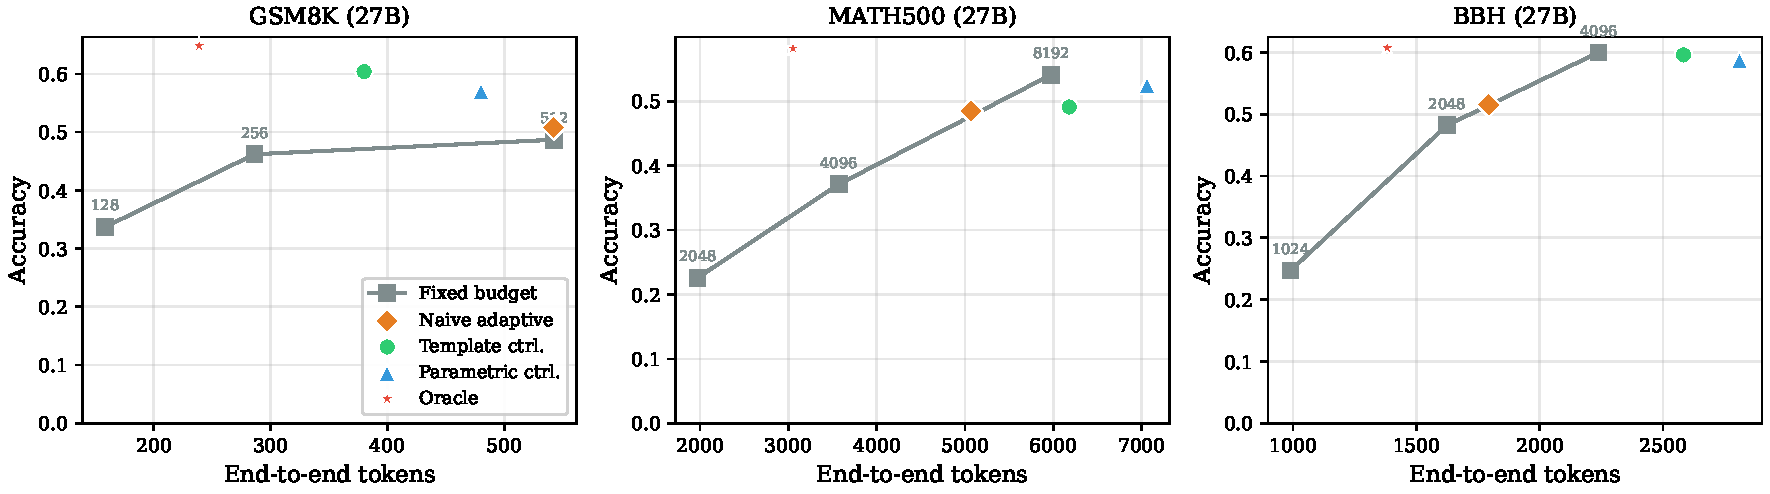
\includegraphics[width=\textwidth]{figures/fig1_pareto_curves.pdf}
\caption{\textbf{Quality--cost Pareto frontiers} on three benchmarks with Qwen3.5-27B. Fixed-budget baselines (gray squares) form the baseline frontier. \adathink{} controllers (colored markers) achieve higher accuracy. Token counts on the $x$-axis include probe overhead for adaptive controllers. The oracle (red star) is a single-pass upper bound.}
\label{fig:pareto-27b}
\end{figure}

\begin{figure}[t]
\centering
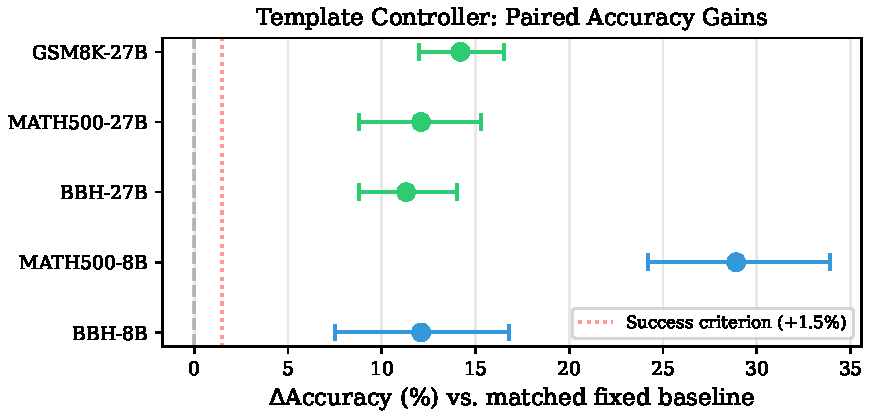
\includegraphics[width=0.65\textwidth]{figures/fig5_significance_forest.pdf}
\caption{\textbf{Statistical significance.} Paired accuracy gains (template controller vs.\ matched fixed baseline) with 95\% bootstrap CIs across all settings. All CIs exclude zero and exceed the $+1.5$\,pp success criterion (red dotted line).}
\label{fig:forest}
\end{figure}

Several observations emerge.
(1)~Gains are consistent across benchmarks ($+11.3$--$14.2$\,pp on 27B, $+12.1$--$28.9$\,pp on 8B), with all CIs excluding zero (Figure~\ref{fig:forest}).
(2)~\textbf{The template controller Pareto-dominates all fixed baselines on GSM8K-27B} (Figure~\ref{fig:pareto-27b}): higher accuracy ($60.4\%$ vs.\ Max-only's $48.7\%$) \emph{and} lower cost ($380.1$ vs.\ $542.7$ tokens).
On MATH500-27B, Max-only achieves higher raw accuracy ($54.1\%$ vs.\ $49.1\%$) because most questions genuinely need extended reasoning, but the template controller still improves utility by $+7.4$\,pp over the mid-tier baseline by routing $25.7\%$ of easy questions to $b_1$.
(3)~The Pareto curves show that no single fixed budget dominates the adaptive controller across the quality--cost frontier.
(4)~Zero-shot cross-benchmark transfer (Appendix~\ref{app:transfer}) shows that templates learned on MATH500 transfer perfectly to BBH ($+13.6$\,pp, matching in-domain), confirming the controller captures a general difficulty pattern rather than overfitting to benchmark-specific artifacts.

\paragraph{Token cost trade-offs.}
The template controller uses more end-to-end tokens than the fixed mid-tier baseline due to probe overhead ($+93.8$ tokens on GSM8K-27B; larger on MATH500/BBH where $b_1$ is higher).
Despite this, \textbf{utility is positive on all five template-controller settings} ($+7.4$--$23.1$\,pp); see Table~\ref{tab:token-deltas} in the Appendix.

\subsection{Ablation Study}
\label{sec:exp:ablation}

To understand which controller components drive the gains, we evaluate restricted variants:
\textbf{Full} uses all budget tiers $\mathcal{B} = \{b_1, b_2, b_3\}$;
\textbf{Halting-only} removes the middle tier ($\mathcal{B} = \{b_1, b_3\}$), testing whether binary easy/hard classification suffices;
\textbf{No-branch} removes the highest tier ($\mathcal{B} = \{b_1, b_2\}$), testing whether upward budget allocation matters;
\textbf{Max-only} and \textbf{Mid-only} are single-budget baselines.

\begin{table}[t]
\centering
\caption{\textbf{Ablation study.} Accuracy and utility under restricted budget sets. Utility for multi-tier variants (Full, Halting-only, No-branch) uses second-pass tokens only; probe overhead is constant across these variants so relative comparisons are valid. Max-only and Mid-only are single-pass (no probe). \textbf{Bold}: best among multi-tier adaptive variants per setting.}
\label{tab:ablation}
\footnotesize
\setlength{\tabcolsep}{3.5pt}
\begin{tabular}{@{}lcccccccccc@{}}
\toprule
& \multicolumn{2}{c}{\textbf{GSM8K-27B}} & \multicolumn{2}{c}{\textbf{M500-27B}} & \multicolumn{2}{c}{\textbf{BBH-27B}} & \multicolumn{2}{c}{\textbf{M500-8B}} & \multicolumn{2}{c}{\textbf{BBH-8B}} \\
\cmidrule(lr){2-3}\cmidrule(lr){4-5}\cmidrule(lr){6-7}\cmidrule(lr){8-9}\cmidrule(lr){10-11}
\textbf{Variant} & Acc & Util & Acc & Util & Acc & Util & Acc & Util & Acc & Util \\
\midrule
Full & \textbf{.621} & \textbf{.541} & .488 & .409 & .590 & .524 & .378 & .270 & .296 & .213 \\
Halting-only & .557 & .440 & \textbf{.507} & \textbf{.427} & \textbf{.596} & \textbf{.530} & \textbf{.403} & \textbf{.292} & \textbf{.314} & \textbf{.226} \\
No-branch & .536 & .467 & .346 & .294 & .466 & .416 & .047 & $-$.005 & .129 & .077 \\
\arrayrulecolor{gray}\midrule\arrayrulecolor{black}
Max-only & .467 & .308 & .541 & .432 & .600 & .518 & .436 & .292 & .325 & .212 \\
Mid-only & .484 & .400 & .371 & .305 & .482 & .423 & .086 & .011 & .171 & .101 \\
\bottomrule
\end{tabular}
\end{table}

Table~\ref{tab:ablation} reveals three patterns.\footnote{Table~\ref{tab:ablation} uses 24 subsets for GSM8K-27B (including one latency subset) vs.\ 23 in Table~\ref{tab:main-gsm8k}; this explains the small discrepancy between Max-only ($46.7\%$) and Fixed-512 ($48.7\%$) across tables.}
(1)~\textbf{Full} wins on GSM8K-27B, but \textbf{Halting-only} is marginally better on MATH500/BBH where the middle tier adds limited value.
(2)~\textbf{No-branch} ($\{b_1, b_2\}$) suffers severely on 8B models ($4.7\%$ on MATH500-8B), confirming that access to $b_K$ is critical.
(3)~\textbf{Max-only} achieves highest accuracy on some settings (e.g., MATH500-27B: $54.1\%$) but at high cost, resulting in lower utility.

\subsection{Latency Analysis}
\label{sec:exp:latency}

Wall-clock latency on A100-80GB (Table~\ref{tab:latency} in the Appendix) reveals a setting-dependent trade-off.
On MATH500-27B and BBH-27B, the adaptive controller reduces latency by $26\%$ and $35\%$ vs.\ the max tier by routing easy questions to lower budgets.
On GSM8K-27B, the two-pass overhead dominates: adaptive latency (34.9\,s) is comparable to the max tier (34.5\,s) because $b_1{=}128$ is small relative to the second pass.
Throughput remains within $5\%$ of fixed baselines, confirming negligible controller decision overhead.

\subsection{Controller Analysis}
\label{sec:exp:analysis}

\paragraph{Value controller penalty sweep.}
The $\rho$ parameter provides a smooth accuracy--cost knob (Figure~\ref{fig:penalty-sweep}): on GSM8K-8B, $\rho{=}0$ yields $+13.6$\,pp at 358 tokens while $\rho{=}0.8$ yields $+4.6$\,pp at 283 tokens.

\paragraph{Oracle gap and why the template works.}
On GSM8K-27B, the template controller achieves $60.4\%$ accuracy vs.\ the oracle's $64.8\%$, closing $76\%$ of the gap between Fixed-256 ($46.2\%$) and the oracle ($64.8\%$).
Feature-stratified analysis (Appendix~\ref{app:why-template}) reveals the mechanism: $\sim$13\% of questions are ``easy'' (correct at $b_1$) with $\sim$60\% overthinking rate at $b_K$; routing them to $b_1$ provides free accuracy.
The remaining gap suggests room for improvement with richer features.

\paragraph{Sensitivity to $\lambda$.}
The template controller is insensitive to $\lambda$ across $[0.05, 0.25]$: the same template is selected for all values and accuracy remains at $60.4\%$ (Table~\ref{tab:lambda-sensitivity} in the Appendix).

\begin{figure}[!htb]
\centering
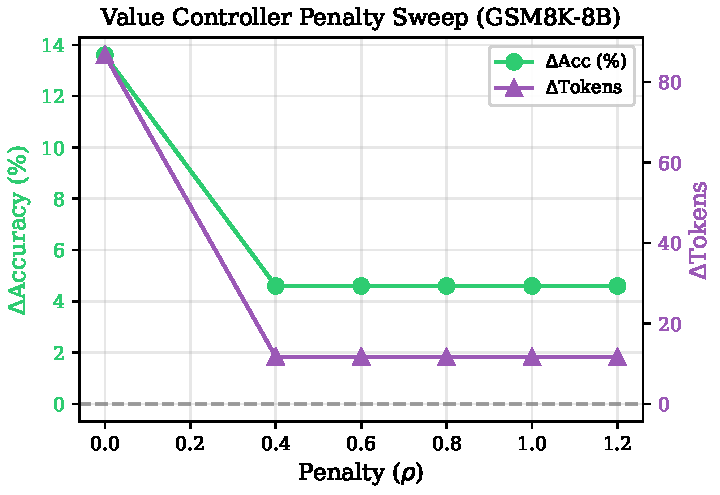
\includegraphics[width=0.48\textwidth]{figures/fig4_penalty_sweep.pdf}
\caption{Value controller penalty sweep on GSM8K-8B (7 seeds, $n=280$). Each point represents a penalty setting $\rho$, showing the accuracy--cost trade-off.}
\label{fig:penalty-sweep}
\end{figure}

\paragraph{Multi-seed robustness.}
Cross-seed standard deviation is \textbf{exactly~0} across all 30 configurations (2 models $\times$ 3 budgets $\times$ 5 algorithm seeds) because greedy decoding is fully deterministic.
The only variance source is the data seed (subset selection), directly captured by the leave-one-subset-out protocol.

\paragraph{Relationship to certainty-guided halting.}
Our difficulty features serve as proxy certainty signals~\citep{aggarwal2023let}: the template controller subsumes simple confidence thresholds by learning the optimal joint mapping.
The naive adaptive baseline (heuristic certainty halting) achieves only $+4.6$\,pp on GSM8K-27B vs.\ the template controller's $+14.2$\,pp.

\paragraph{Error taxonomy.}
Classifying errors as under-budget, over-budget (overthinking), or intrinsic reveals that over-budget errors dominate on GSM8K-27B ($41.2\%$) while intrinsic errors dominate on BBH-27B ($61.8\%$), indicating near-optimal routing on harder tasks (Appendix~\ref{app:error-taxonomy}).

\paragraph{Comparison scope.}
\adathink{} operates in a strictly \emph{inference-only} setting: it requires no fine-tuning, reward modeling, or access to training data.
Training-time approaches such as SelfBudgeter~\citep{liu2025selfbudgeter}, BudgetThinker~\citep{yang2025budgetthinker}, and TALE~\citep{han2025tale} can internalize budget decisions into the model and likely achieve higher accuracy, but they require substantial compute for data curation and RL/SFT training, which limits direct comparison.
ThoughtTerminator~\citep{muennighoff2025thoughtterminator} is the closest inference-time baseline; however, its early-stopping mechanism differs from our budget-selection framework and its codebase targets different model families.
Our results establish what is achievable \emph{without any model modification}---a lower bound that training-time methods should be compared against to quantify the value of their additional compute investment.

\section{Conclusion}
\label{sec:conclusion}

We presented \adathink{}, a training-free, inference-only framework for adaptive test-time compute allocation that exploits a fundamental property of LLM reasoning: \emph{fixed budgets create structured compute heterogeneity}, systematically overthinking easy questions and undercomputing hard ones.

Our primary empirical contribution is demonstrating that this heterogeneity is so regular that a lookup table over three binary difficulty features---answer presence, token utilization, and answer consistency---closes $76\%$ of the gap to an oracle budget selector.
The template controller achieves $+11.3$--$28.9$\,pp accuracy gains and $+7.4$--$23.1$\,pp utility gains across three benchmarks and two Qwen model scales, with all improvements statistically significant.
Feature-stratified analysis reveals the mechanism: $\sim$13\% of questions are easy (with $\sim$60\% overthinking rate at $b_K$), while $\sim$60\% are hard and benefit from escalation.
Cross-benchmark transfer (MATH500$\to$BBH: $+13.6$\,pp, matching in-domain) confirms the difficulty pattern generalizes across reasoning domains.

\paragraph{Limitations.}
(1)~All experiments use Qwen-family models; while the underlying phenomenon (overthinking) is well-documented across model families, we have not validated our specific controller on non-Qwen architectures.
(2)~The two-pass design incurs overhead on $69.7\%$ of GSM8K-27B questions; naive prefix reuse underperforms fresh re-generation ($52.5\%$ vs.\ $60.4\%$), motivating smarter continuation strategies.
(3)~Evaluation covers mathematical and logical reasoning; generalization to code generation and open-ended QA is untested.
(4)~Direct comparison to training-time approaches (SelfBudgeter, BudgetThinker) requires fine-tuning outside our inference-only scope.

\paragraph{Broader impact.}
By reducing unnecessary compute in LLM reasoning, \adathink{} can lower inference costs and energy consumption at scale.

\paragraph{Future work.}
Key directions include cross-family validation (Llama, Mistral), lightweight difficulty classifiers (e.g., logprob trends) to eliminate the probe pass, partial-trace reuse via KV-cache prefix seeding, and integration with training-time approaches as a complementary post-hoc refinement layer.


\bibliographystyle{plainnat}
\bibliography{references}

\section*{NeurIPS Paper Checklist}

\begin{enumerate}

\item {\bf Claims}
    \begin{enumerate}
        \item Do the main claims made in the abstract and introduction accurately reflect the paper's contributions and scope?
        \answerYes{All accuracy and token-cost claims are derived from reproducible experiments with fixed seeds (Appendix~\ref{app:reproducibility}). The coupling tax is demonstrated across three model sizes (8B, 9B, 27B) within the Qwen3 family, with auxiliary validation on DeepSeek-R1, and two benchmarks (GSM8K, MATH-500). \method{} evaluation uses per-sample matched data (Table~\ref{tab:main-results}). Claims about generality are scoped to the validated models and benchmarks (\S\ref{sec:conclusion}).}
    \end{enumerate}

\item {\bf Limitations}
    \begin{enumerate}
        \item Does the paper discuss the limitations of the work performed by the authors?
        \answerYes{The conclusion (\S\ref{sec:conclusion}) discusses limitations including the focus on mathematical reasoning benchmarks, the binary routing signal (vs.\ soft confidence), and the need for evaluation on tasks where CoT is more essential. The discussion (\S\ref{sec:discussion}) further analyzes scope limitations, the format-vs-information tax distinction, and deployment criteria.}
    \end{enumerate}

\item {\bf Theory}
    \begin{enumerate}
        \item Does the paper include theoretical results?
        \answerYes{Section~\ref{sec:theory} presents an analytical framework. The truncation-waste decomposition (Eq.~\ref{eq:acc-decomp}) expresses thinking-mode accuracy as a function of the chain-length CDF and conditional accuracies; Theorem~\ref{thm:mrsd-pareto} shows \method{} achieves a Pareto improvement over fixed-mode strategies under a net recovery condition. The crossover budget formula (Eq.~\ref{eq:crossover}) and inverse-scaling analysis (Appendix~\ref{app:theory-full}) complete the framework. All derivations are in the main text and appendix.}
    \end{enumerate}

\item {\bf Experiments}
    \begin{enumerate}
        \item Does the paper include experiments?
        \answerYes{Sections~\ref{sec:thinking-tax} and \ref{sec:experiments} report comprehensive experiments across GSM8K (full set, $n{=}1{,}319$) and MATH-500, with the Qwen3 family (primary) and auxiliary DeepSeek-R1 validation.}
        \item Does the paper report error bars or confidence intervals?
        \answerYes{We report 95\% bootstrap confidence intervals (10{,}000 resamples) for key comparisons in Table~\ref{tab:main-results} and the failure decomposition table. Since we use deterministic (greedy) decoding on fixed test sets, residual variance comes from cross-hardware floating-point nondeterminism rather than stochastic generation (Appendix~\ref{app:reproducibility}). Cross-seed validation for DeepSeek-R1 uses 5 data seeds (Appendix~\ref{app:deepseek}).}
        \item Does the paper report the number of parameters, FLOPs, or other computational cost?
        \answerYes{Average token counts are reported in all tables. Model sizes (8B, 9B, 27B) are specified throughout.}
        \item Does the paper report the computational cost of the experiments?
        \answerYes{Appendix~\ref{app:reproducibility} reports approximately 200 A100-GPU-hours total compute.}
    \end{enumerate}

\item {\bf Reproducibility}
    \begin{enumerate}
        \item Does the paper include the code, data, and instructions needed to reproduce the main experimental results?
        \answerYes{Appendix~\ref{app:experimental_details} provides complete hardware, software, budget control mechanism, and answer extraction pipeline details. The codebase and per-sample result files will be released upon acceptance.}
        \item Does the paper report all the main experimental details needed to understand the results?
        \answerYes{Budget control via \texttt{max\_new\_tokens}, greedy decoding ($\tau{=}0$), answer extraction pipeline, dataset splits, and random seeds are fully specified in Appendix~\ref{app:experimental_details}.}
    \end{enumerate}

\item {\bf Open access to data and code}
    \begin{enumerate}
        \item Does the paper promise to release code and/or data?
        \answerYes{We will release the complete codebase, per-sample result CSVs, and \method{} implementation scripts.}
    \end{enumerate}

\item {\bf Experimental Setting/Details}
    \begin{enumerate}
        \item Does the paper specify the computing infrastructure used for running the experiments?
        \answerYes{NVIDIA A100-80GB GPUs, PyTorch 2.4.1 (CUDA 12.4), HuggingFace Transformers 5.5.0, bfloat16 precision (Appendix~\ref{app:experimental_details}).}
        \item Does the paper specify all the training and test details necessary to reproduce the results?
        \answerYes{No training is performed---\method{} is a training-free inference method. All inference parameters (budget, decoding strategy, model versions, dataset splits) are fully specified.}
    \end{enumerate}

\item {\bf Broader Impacts}
    \begin{enumerate}
        \item Does the paper discuss potential broader impacts of their work?
        \answerYes{The conclusion discusses practical implications for LLM deployment: defaulting to non-thinking mode at constrained budgets can simultaneously improve accuracy and reduce computational cost, benefiting both providers and users. Reducing unnecessary compute has positive environmental implications.}
    \end{enumerate}

\item {\bf Safeguards}
    \begin{enumerate}
        \item Does the paper describe safeguards for responsible use?
        \answerNA{Our work optimizes inference efficiency for standard reasoning benchmarks and does not introduce new capabilities requiring specific safeguards.}
    \end{enumerate}

\item {\bf Licenses}
    \begin{enumerate}
        \item Are the creators of assets used in the paper properly credited?
        \answerYes{GSM8K~\citep{cobbe2021gsm8k}, MATH~\citep{hendrycks2021math}, Qwen3~\citep{qwen3_2025}, and DeepSeek-R1~\citep{deepseekr1} are properly cited. All models are publicly available under their respective licenses.}
    \end{enumerate}

\item {\bf New Assets}
    \begin{enumerate}
        \item Are new assets introduced in the paper well documented?
        \answerYes{The \method{} inference scripts and per-sample result files will be released with documentation.}
    \end{enumerate}

\item {\bf Human Subjects}
    \begin{enumerate}
        \item Does the paper involve crowdsourcing or human subjects?
        \answerNo{}
    \end{enumerate}

\end{enumerate}


\appendix
\section{Reproducibility Details}
\label{app:reproducibility}

\subsection{Hardware and Software}
All experiments were conducted on NVIDIA A100-80GB GPUs.
Models were loaded in \texttt{bfloat16} precision using HuggingFace Transformers.
The codebase uses Python 3.10, PyTorch 2.5.1 (CUDA 12.4), and Transformers 4.46.0.

\subsection{Seed Protocol}
Each experiment is parameterized by two independent random seeds:
\begin{itemize}[nosep,leftmargin=*]
    \item \textbf{Algorithm seed} (\texttt{seed}): controls model sampling randomness. Fixed at 11 for most experiments.
    \item \textbf{Data seed} (\texttt{data\_seed}): controls the random subset of questions selected from the benchmark. Varied across replications.
\end{itemize}
This decoupling ensures that performance differences across replications reflect genuine question-set variability rather than sampling noise.

\subsection{Replication Counts}

\begin{table}[h]
\centering
\caption{Replication details per benchmark--model combination.}
\small
\begin{tabular}{@{}lcccc@{}}
\toprule
\textbf{Setting} & \textbf{Model} & \textbf{Subsets} & $n$ \textbf{per subset} & \textbf{Total} $n$ \\
\midrule
GSM8K & Qwen3.5-27B & 23 & 40 & 920 \\
GSM8K & Qwen3.5-27B & 24 (latency) & 40 & 960 \\
MATH500 & Qwen3.5-27B & 17 & 40 & 680 \\
BBH & Qwen3.5-27B & 17 & 40 & 680 \\
GSM8K & Qwen3-8B (think) & 7 & 40 & 280 \\
MATH500 & Qwen3-8B (think) & 9 & 40 & 360 \\
BBH & Qwen3-8B (think) & 7 & 40 & 280 \\
\bottomrule
\end{tabular}
\end{table}

\subsection{Parser and Measurement Details}
For long-thinking models (especially Qwen3.5-27B), generations often lack an explicit ``Final answer'' within the token limit.
We employ two complementary strategies:
\begin{itemize}[nosep,leftmargin=*]
    \item \textbf{Strict final-answer parsing} (\texttt{strict\_final\_only}): only counts answers that appear in the expected format. Questions without a parseable answer receive a score of 0.
    \item \textbf{Projection on missing final} (\texttt{projection\_on\_missing\_final}): when no final answer is found within the budget, extends generation by up to 16 additional tokens to allow answer completion.
\end{itemize}

\subsection{Template Controller Training Details}
The template controller is trained with $\lambda = 0.15$ for the utility objective.
Token costs are normalized by the maximum budget $b_K$ for each benchmark.
Leave-one-subset-out cross-validation iterates over all subsets; the template with highest training utility is applied to the held-out subset.
The search space is $|\mathcal{B}|^D$ possible templates, which is small enough ($\leq 3^8 = 6561$) for exhaustive enumeration.

\subsection{Bootstrap Confidence Intervals}
All reported confidence intervals use 10,000 bootstrap resamples with a fixed bootstrap seed (20260228) for reproducibility.
We use the percentile method on paired per-sample deltas (adaptive minus fixed baseline) to construct 95\% CIs.

\section{Additional Results}
\label{app:additional}

\subsection{Self-Consistency and Continuation Baselines}
\label{app:fair-sc}

Table~\ref{tab:fair-sc} provides a comprehensive comparison of self-consistency variants and the continuation-from-$b_1$ baseline on GSM8K-27B.
All SC variants use $T{=}0.7$, majority vote, and total budget $\leq 512$ tokens.
SC@8$\times$64 achieves only $4.5\%$ because 64 tokens is insufficient for the 27B model in thinking mode; SC@2$\times$256 collapses ($7.5\%$) because $K{=}2$ provides insufficient diversity.
SC@4$\times$128 is the strongest SC baseline at $42.5\%$, still far below the template controller ($60.4\%$).

\begin{table}[ht]
\centering
\caption{\textbf{Fair SC and continuation baselines} on GSM8K-27B ($n{=}40$, data seed 42). All SC variants use $T{=}0.7$, majority vote, and total budget $\leq 512$ tokens.}
\label{tab:fair-sc}
\small
\begin{tabular}{@{}lccc@{}}
\toprule
\textbf{Method} & \textbf{Accuracy} & \textbf{Avg.\ Tokens} & \textbf{Parse Rate} \\
\midrule
SC@8$\times$64 & 0.045 & 512 & 0.05 \\
SC@2$\times$256 & 0.075 & 505 & 1.00 \\
SC@4$\times$128 & 0.425 & 512 & 1.00 \\
SC@1$\times$512 ($T{=}0.7$) & 0.375 & 444 & 1.00 \\
\midrule
Fixed-512 ($T{=}0$) & 0.487 & 543 & -- \\
Continuation-from-$b_1$ & 0.525 & 479.9 & -- \\
\textbf{Template ctrl.} & \textbf{0.604} & \textbf{380.1} & -- \\
\bottomrule
\end{tabular}
\end{table}

\subsection{Why the Template Controller Works}
\label{app:why-template}

The three difficulty features partition questions into strata with dramatically different accuracy profiles across budgets, enabling effective per-stratum routing.
Table~\ref{tab:feature-analysis} shows this for MATH500-27B and BBH-27B.

\begin{table}[ht]
\centering
\caption{\textbf{Feature-stratified accuracy} across budget tiers. ``Easy'' questions (consistent answer at low utilization) achieve 90+\% at $b_1$ but \emph{drop} at $b_K$ due to overthinking. ``Hard'' questions (no answer, high utilization) gain substantially from $b_K$.}
\label{tab:feature-analysis}
\small
\begin{tabular}{@{}lcrrrrl@{}}
\toprule
\textbf{Setting} & \textbf{Pattern} & \textbf{Frac.} & \textbf{Acc@}$b_1$ & \textbf{Acc@}$b_K$ & $\Delta$ & \textbf{Interpretation} \\
\midrule
\multirow{3}{*}{MATH500-27B} & $(1,0,1)$ & 13\% & 92.3 & 37.2 & $-$55.1 & Easy: b1 suffices \\
 & $(1,1,0)$ & 27\% & 42.0 & 27.1 & $-$14.9 & Medium: overthinks \\
 & $(0,1,0)$ & 60\% & 0.0 & 18.9 & $+$18.9 & Hard: needs b$_K$ \\
\midrule
\multirow{3}{*}{BBH-27B} & $(1,0,1)$ & 14\% & 90.5 & 47.1 & $-$43.4 & Easy: b1 suffices \\
 & $(1,1,0)$ & 42\% & 28.2 & 24.2 & $-$4.0 & Medium: slight overthink \\
 & $(0,1,0)$ & 44\% & 0.0 & 30.1 & $+$30.1 & Hard: needs b$_K$ \\
\bottomrule
\end{tabular}
\end{table}

Three mechanisms drive the template's effectiveness:
(1)~\textbf{Overthinking prevention}: 13--14\% of questions are ``easy'' (correct and consistent at $b_1$).
Extending these to $b_K$ \emph{halves} their accuracy (59.7\% overthinking rate on MATH500-27B), so routing them to $b_1$ provides a large, free accuracy gain.
(2)~\textbf{Hard-question escalation}: 44--60\% of questions produce no answer at $b_1$. These benefit from $b_K$ (+18.9/+30.1\,pp), so routing them upward is critical.
(3)~\textbf{The feature space is compact}: with $\leq 8$ categories, the template avoids overfitting even with modest training data (40 questions per subset), unlike higher-dimensional feature spaces.

\subsection{Overthinking Evidence}
\label{app:overthinking}

Table~\ref{tab:overthinking} summarizes the overthinking phenomenon across all benchmark--model combinations.
In all cases, the naive adaptive policy (heuristic early stopping) achieves accuracy comparable to or slightly above the maximum-budget fixed baseline but at similar cost, confirming that purely heuristic adaptation provides limited benefit.

\begin{table}[ht]
\centering
\caption{Overthinking evidence: accuracy at each fixed budget and under naive adaptive control.}
\label{tab:overthinking}
\small
\begin{tabular}{@{}llccccc@{}}
\toprule
\textbf{Benchmark} & \textbf{Model} & \textbf{Low} & \textbf{Mid} & \textbf{High} & \textbf{Adaptive} & $\Delta$\textbf{(High$-$Mid)} \\
\midrule
GSM8K & 27B & .337 & .462 & .487 & .508 & +.025 \\
MATH500 & 27B & .226 & .371 & .541 & .485 & +.170 \\
BBH & 27B & .247 & .482 & .600 & .515 & +.118 \\
MATH500 & 8B & .006 & .086 & .436 & .425 & +.350 \\
BBH & 8B & .036 & .171 & .325 & .321 & +.154 \\
\bottomrule
\end{tabular}
\end{table}

\subsection{Full Controller Comparison}
\label{app:full-comparison}

Table~\ref{tab:full-comparison} provides a complete comparison of all controller types across all settings.

\begin{table}[ht]
\centering
\caption{Full controller comparison across all benchmark--model combinations. Utility values include end-to-end probe overhead for all adaptive controllers. Oracle is single-pass (no probe).}
\label{tab:full-comparison}
\small
\begin{tabular}{@{}llcccc@{}}
\toprule
\textbf{Benchmark} & \textbf{Model} & \textbf{Template} & \textbf{Parametric} & \textbf{Value (best)} & \textbf{Oracle$^\dagger$} \\
\midrule
\multicolumn{6}{c}{\textit{Accuracy}} \\
\midrule
GSM8K & 27B & .604 & .570 & .514 & .648 \\
MATH500 & 27B & .491 & .525 & .515 & .582 \\
BBH & 27B & .596 & .588 & .579 & .607 \\
MATH500 & 8B & .375 & .436 & .436 & .439 \\
BBH & 8B & .293 & .304 & .282 & .346 \\
\midrule
\multicolumn{6}{c}{\textit{End-to-end Utility ($\lambda=0.15$)}} \\
\midrule
GSM8K & 27B & .493 & .431 & .411 & .579 \\
MATH500 & 27B & .378 & .396 & .400 & .526 \\
BBH & 27B & .501 & .485 & .484 & .557 \\
MATH500 & 8B & .240 & .266 & .267 & .362 \\
BBH & 8B & .178 & .189 & .185 & .293 \\
\bottomrule
\multicolumn{6}{@{}l}{\footnotesize $^\dagger$Oracle: single-pass upper bound (no probe overhead).}
\end{tabular}
\end{table}

\subsection{Value Controller Penalty Sweep}
\label{app:penalty-sweep}

Table~\ref{tab:penalty-sweep-full} provides the full penalty sweep for the value-based controller on GSM8K-8B (7 seeds, $n=280$).
The identical results for $\rho \in [0.4, 1.2]$ reflect the discrete nature of the budget set: once $\rho$ exceeds the threshold where the argmax in \eqref{eq:value-decision} switches from the highest to the middle tier, further increases do not change the selected budget until a second transition point (which lies beyond $\rho = 1.2$ for this data).

\begin{table}[ht]
\centering
\caption{Value controller penalty sweep on GSM8K-8B vs.\ Fixed-256.}
\label{tab:penalty-sweep-full}
\small
\begin{tabular}{@{}ccccc@{}}
\toprule
$\rho$ & $\Delta$\textbf{Acc} & \textbf{95\% CI} & $\Delta$\textbf{Tokens} & $\Delta$\textbf{Utility} \\
\midrule
0.0 & +13.6\,pp & $[+9.3, +18.2]$ & +86.7 & +11.0\,pp \\
0.4 & +4.6\,pp & $[+0.7, +8.6]$ & +11.7 & +4.3\,pp \\
0.6 & +4.6\,pp & $[+0.7, +8.6]$ & +11.7 & +4.3\,pp \\
0.8 & +4.6\,pp & $[+0.7, +8.6]$ & +11.7 & +4.3\,pp \\
1.0 & +4.6\,pp & $[+0.7, +8.6]$ & +11.7 & +4.3\,pp \\
1.2 & +4.6\,pp & $[+0.7, +8.6]$ & +11.7 & +4.3\,pp \\
\bottomrule
\end{tabular}
\end{table}

\subsection{Quality--Cost Frontiers for 8B Models}
\label{app:pareto-8b}

Figure~\ref{fig:pareto-8b} extends the Pareto frontier analysis to Qwen3-8B.
The adaptive controllers consistently outperform fixed baselines on both benchmarks, with particularly large gains on MATH500 where the fixed mid-tier baseline achieves only $8.6\%$ accuracy.

\begin{figure}[ht]
\centering
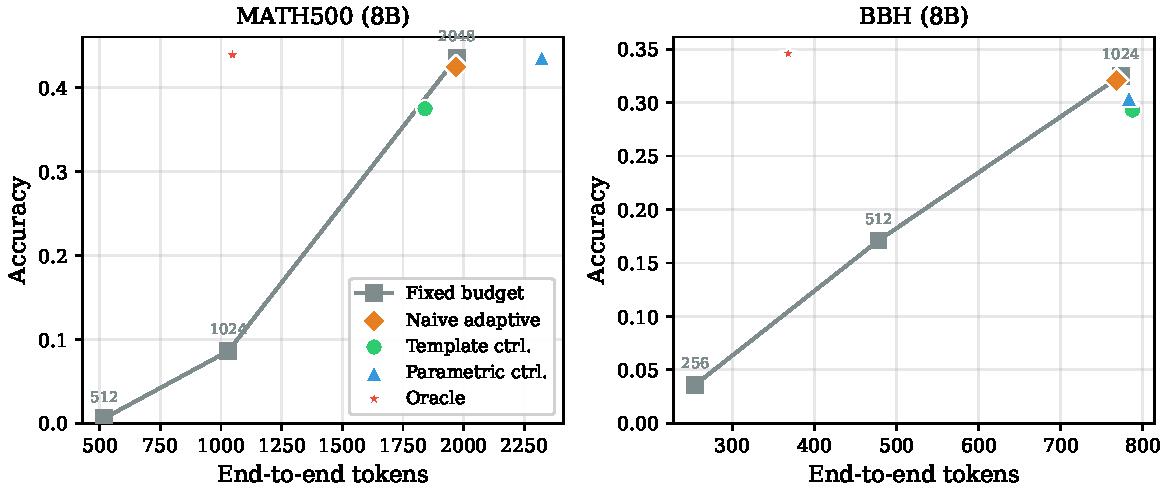
\includegraphics[width=\textwidth]{figures/fig2_pareto_8b.pdf}
\caption{Quality--cost Pareto frontiers for Qwen3-8B on MATH500 and BBH. Token counts include probe overhead for adaptive controllers. The adaptive controllers achieve substantially higher accuracy than fixed baselines.}
\label{fig:pareto-8b}
\end{figure}

\subsection{Budget Allocation Distribution}
\label{app:budget-alloc}

Figure~\ref{fig:budget-alloc} visualizes the template controller's budget allocation across all settings.
On GSM8K-27B, $30\%$ of questions are routed to the lowest tier, $61\%$ to the middle tier, and only $9\%$ to the highest tier, confirming that the controller actively differentiates questions rather than defaulting to a single budget.
On harder benchmarks (MATH500, BBH), a larger fraction of questions are routed to the highest tier, consistent with the models requiring more reasoning tokens.

\begin{figure}[ht]
\centering
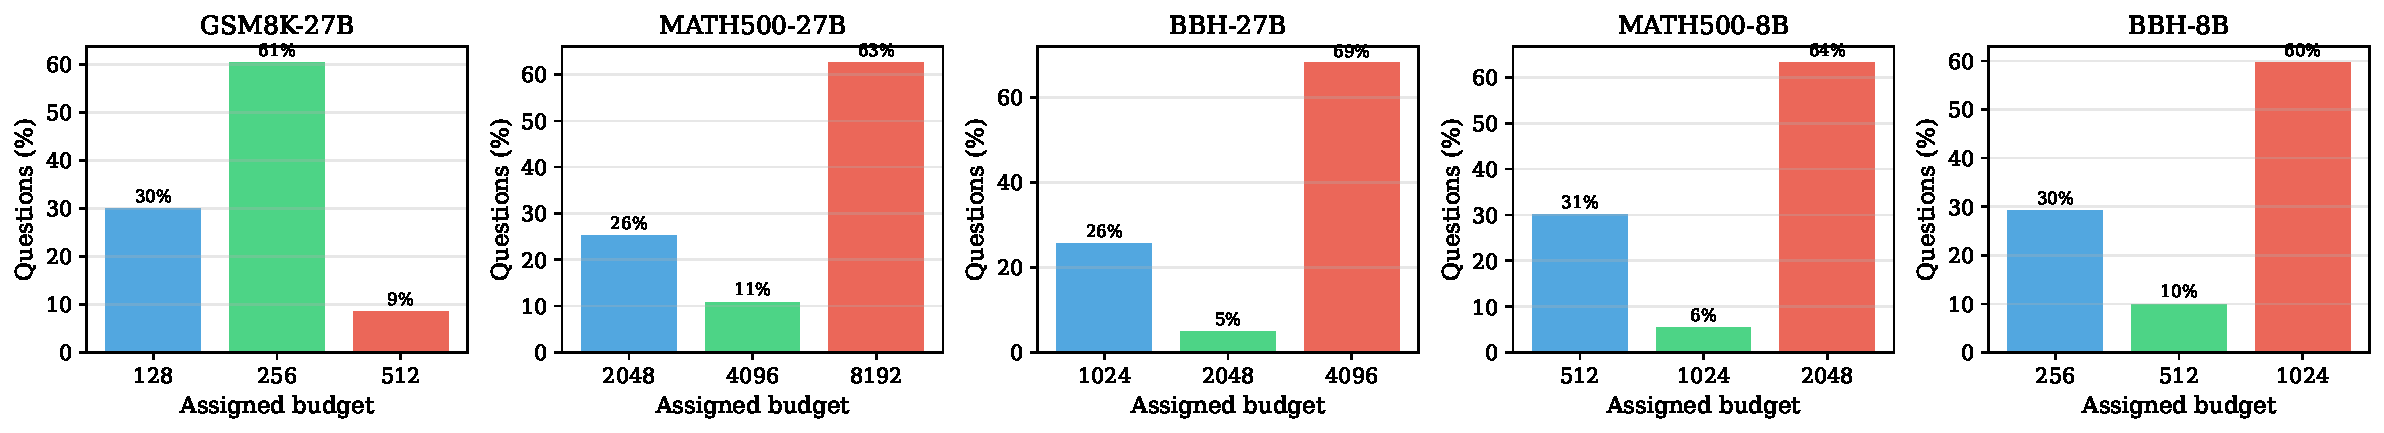
\includegraphics[width=0.8\textwidth]{figures/fig7_budget_allocation.pdf}
\caption{Template controller budget allocation distribution across all benchmark--model settings. The controller routes different fractions of questions to each tier depending on benchmark difficulty.}
\label{fig:budget-alloc}
\end{figure}

\subsection{Error Taxonomy}
\label{app:error-taxonomy}

To understand \emph{why} the controller fails, we classify all incorrect predictions into three categories (Figure~\ref{fig:error-taxonomy}):
(1)~\textbf{Under-budget}: the controller assigned too few tokens---a larger budget would have yielded a correct answer;
(2)~\textbf{Over-budget}: the controller assigned more tokens than needed---the question was answered correctly at a lower tier but not at the assigned one (overthinking);
(3)~\textbf{Intrinsic}: the controller chose the oracle-optimal budget, but the model still answered incorrectly.

On GSM8K-27B, under-budget errors account for $31.3\%$ and over-budget errors for $41.2\%$, with intrinsic errors at $27.5\%$.
The over-budget dominance confirms that even the learned controller still suffers from residual overthinking.
On BBH-27B, intrinsic errors dominate ($61.8\%$), indicating that the controller's budget selection is near-optimal but the model's fundamental capability limits accuracy.

\begin{figure}[ht]
\centering
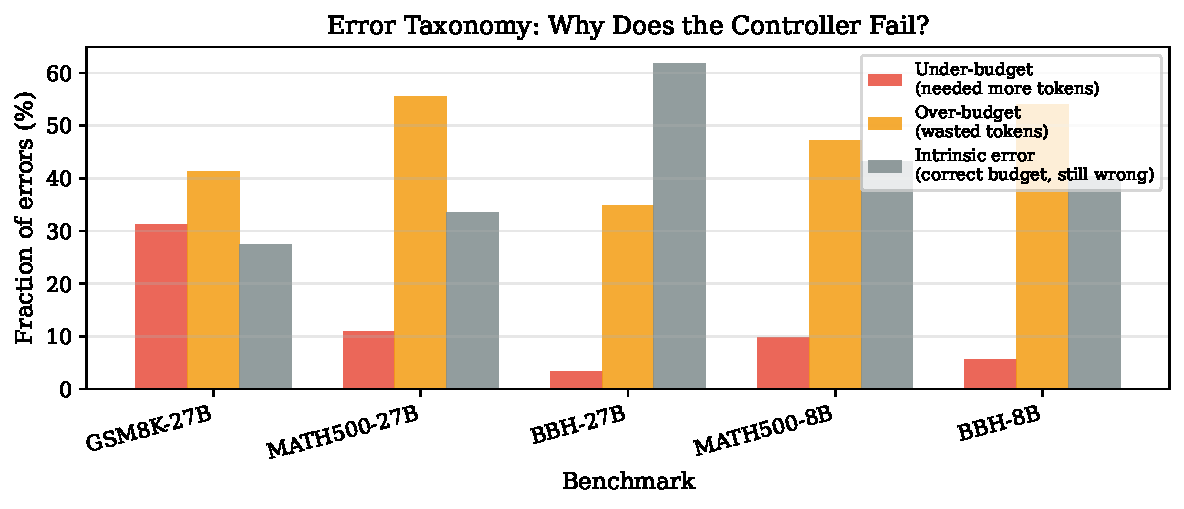
\includegraphics[width=0.8\textwidth]{figures/fig6_error_taxonomy.pdf}
\caption{\textbf{Error taxonomy} across all benchmark--model settings. Under-budget errors (model needed more tokens), over-budget errors (model overthought), and intrinsic errors (correct budget, still wrong).}
\label{fig:error-taxonomy}
\end{figure}

\subsection{Wall-Clock Latency}
\label{app:latency}

\begin{table}[ht]
\centering
\caption{\textbf{Wall-clock latency.} Mean latency (seconds) and throughput (tokens/s) across budgets and adaptive control on A100-80GB.}
\label{tab:latency}
\small
\begin{tabular}{@{}lcccccc@{}}
\toprule
& \multicolumn{2}{c}{\textbf{Baseline ($b_2$)}} & \multicolumn{2}{c}{\textbf{Max ($b_K$)}} & \multicolumn{2}{c}{\textbf{Adaptive}} \\
\cmidrule(lr){2-3}\cmidrule(lr){4-5}\cmidrule(lr){6-7}
\textbf{Setting} & Lat.\ (s) & Thr. & Lat.\ (s) & Thr. & Lat.\ (s) & Thr. \\
\midrule
GSM8K-27B & 18.3 & 15.6 & 34.5 & 15.7 & 34.9 & 15.5 \\
MATH500-27B & 2.8 & 1254.5 & 5.7 & 1041.6 & 4.2 & 1217.2 \\
BBH-27B & 1.4 & 1181.8 & 2.6 & 858.9 & 1.7 & 1053.0 \\
MATH500-8B & 3.4 & 305.7 & 6.4 & 310.2 & 6.5 & 302.4 \\
BBH-8B & 0.17 & 2865.3 & 0.34 & 2293.5 & 0.33 & 2365.7 \\
\bottomrule
\end{tabular}
\end{table}

\subsection{Token Cost Deltas Across All Settings}
\label{app:token-deltas}

Table~\ref{tab:token-deltas} reports end-to-end token consumption for the template controller versus the matched fixed-budget (mid-tier) baseline across all settings.
Tokens include the probe-pass cost for questions routed to $b^* > b_1$ (Algorithm~\ref{alg:adathink}).
The controller uses more tokens than the fixed baseline in all settings due to the two-pass overhead.
Despite this, utility gains are positive on all settings because accuracy improvements outweigh the cost penalty.

\begin{table}[ht]
\centering
\caption{End-to-end token cost comparison: template controller vs.\ fixed mid-tier baseline. Ctrl Tok includes probe overhead for questions with $b^* > b_1$. $\Delta$Acc and $\Delta$Util in pp.}
\label{tab:token-deltas}
\small
\begin{tabular}{@{}llrrrrr@{}}
\toprule
\textbf{Bench.} & \textbf{Model} & \textbf{Ctrl Tok} & \textbf{Fixed Tok} & $\Delta$\textbf{Tok} & $\Delta$\textbf{Acc (pp)} & $\Delta$\textbf{Util (pp)} \\
\midrule
GSM8K & 27B & 380.1 & 286.3 & +93.8 & +14.2 & +11.5 \\
MATH500 & 27B & 6102.6 & 3570.4 & +2532.2 & +12.1 & +7.4 \\
BBH & 27B & 2526.5 & 1624.1 & +902.4 & +11.3 & +8.0 \\
MATH500 & 8B & 1823.0 & 1030.0 & +793.0 & +28.9 & +23.1 \\
BBH & 8B & 763.9 & 478.0 & +285.9 & +12.1 & +8.0 \\
\bottomrule
\end{tabular}
\end{table}

\subsection{Two-Pass Overhead Quantification}
\label{app:two-pass}

Table~\ref{tab:two-pass} quantifies the two-pass overhead across all settings.
When the controller assigns $b^* = b_1$, the initial trace is reused directly (no overhead).
When $b^* > b_1$, a fresh second pass is required; the probe tokens are fully wasted.
The ``$\mathbb{E}[\text{overhead}]$'' column reports the expected probe waste, computed as $P(b^* > b_1) \times \bar{t}(b_1)$ where $\bar{t}(b_1)$ is the average probe-pass token count.
All end-to-end token counts in Tables~\ref{tab:main-gsm8k}, \ref{tab:cross}, and \ref{tab:token-deltas} include this overhead.

\begin{table}[ht]
\centering
\caption{Two-pass overhead. ``Stay $b_1$'' is the fraction of questions reused from the first pass. ``Worst ($b_K$)'' is the fraction routed to the maximum tier.}
\label{tab:two-pass}
\small
\begin{tabular}{@{}llccccc@{}}
\toprule
\textbf{Benchmark} & \textbf{Model} & $b_1$ & $b_K$ & \textbf{Stay $b_1$} & \textbf{Worst ($b_K$)} & $\mathbb{E}[\textbf{overhead}]$ \\
\midrule
GSM8K & 27B & 128 & 512 & 30.3\% & 8.9\% & 111 tok \\
MATH500 & 27B & 2048 & 8192 & 25.7\% & 62.9\% & 1545 tok \\
BBH & 27B & 1024 & 4096 & 26.0\% & 68.5\% & 781 tok \\
MATH500 & 8B & 512 & 2048 & 30.6\% & 63.6\% & 378 tok \\
BBH & 8B & 256 & 1024 & 29.6\% & 60.0\% & 203 tok \\
\bottomrule
\end{tabular}
\end{table}

Two observations are noteworthy.
First, on GSM8K-27B the overhead is modest ($111$ tokens, $\sim\!22\%$ of $b_K$) because $b_1$ is small and many questions are handled in a single pass.
Second, on MATH500 and BBH the overhead is substantial ($378$--$1545$ tokens) because $b_1$ is itself large; these are the settings where partial-trace reuse would yield the greatest latency and cost savings.

\subsection{Value Controller Calibration}
\label{app:value-calibration}

To assess whether the value-based controller's correctness estimates are well-calibrated, we partition GSM8K-8B questions ($n=280$, $\rho=0$) by their estimated low-budget correctness probability $\hat{V}(x, b_1)$ into three strata.
Table~\ref{tab:calibration} shows that the controller's budget decisions align well with difficulty: questions with high estimated correctness receive lower budgets and achieve perfect accuracy, while questions with low estimates are routed to higher budgets.

\begin{table}[ht]
\centering
\caption{Value controller calibration on GSM8K-8B ($\rho=0$). Questions are stratified by the estimated correctness probability at $b_1$.}
\label{tab:calibration}
\small
\begin{tabular}{@{}lcccc@{}}
\toprule
\textbf{Stratum} & $n$ & \textbf{Acc.} & \textbf{Avg.\ Budget} & \textbf{128/256/512} \\
\midrule
Low ($\hat{V}{<}0.3$) & 84 & .631 & 440 & 6/19/75\% \\
Mid ($0.3{\leq}\hat{V}{<}0.7$) & 171 & .778 & 343 & 6/57/37\% \\
High ($\hat{V}{\geq}0.7$) & 25 & 1.00 & 159 & 76/24/0\% \\
\bottomrule
\end{tabular}
\end{table}

We note two limitations of the current calibration.
First, category-level sparsity can affect estimate quality: the ``high'' stratum contains only 25 questions, and rare difficulty categories at extreme budgets may have fewer than 10 training instances per fold.
Our fallback to the corpus-wide mean for categories with $<5$ samples mitigates but does not eliminate this concern.
Second, calibration is evaluated on the same benchmark distribution used for training; generalization to shifted distributions (e.g., different difficulty mixes) would require recollection of traces.

\subsection{Sensitivity to $\rho$ Across Benchmarks}
\label{app:rho-sensitivity}

Table~\ref{tab:rho-multi} extends the value-controller penalty sweep from GSM8K-8B (Table~\ref{tab:penalty-sweep-full}) to MATH500-27B and BBH-27B.
On GSM8K-8B, $\rho$ provides a smooth accuracy--cost knob (75.4\% at 358 tokens down to 66.4\% at 283 tokens).
On MATH500-27B the trade-off is also clear ($51.5\% \to 46.6\%$ accuracy, $4723 \to 3829$ tokens).
On BBH-27B the effect is smaller ($57.9\% \to 56.8\%$), suggesting that most questions on BBH genuinely need the higher budget and there is less room for cost reduction.

\begin{table}[ht]
\centering
\caption{Value controller $\rho$ sensitivity across benchmarks. All accuracy and utility values are absolute (not deltas).}
\label{tab:rho-multi}
\small
\begin{tabular}{@{}cccc|ccc|ccc@{}}
\toprule
& \multicolumn{3}{c|}{\textbf{GSM8K-8B}} & \multicolumn{3}{c|}{\textbf{MATH500-27B}} & \multicolumn{3}{c}{\textbf{BBH-27B}} \\
$\rho$ & Acc & Tok & Util & Acc & Tok & Util & Acc & Tok & Util \\
\midrule
0.0 & .754 & 358 & .649 & .515 & 4723 & .428 & .579 & 1805 & .513 \\
0.2 & .711 & 314 & .619 & -- & -- & -- & -- & -- & -- \\
0.4 & .704 & 310 & .613 & .482 & 4105 & .407 & .571 & 1784 & .505 \\
0.6 & .682 & 296 & .595 & -- & -- & -- & -- & -- & -- \\
0.8 & .664 & 283 & .581 & .466 & 3829 & .396 & .568 & 1770 & .503 \\
\bottomrule
\end{tabular}
\end{table}

\paragraph{Robustness to $\lambda$.}
We fix $\lambda = 0.15$ throughout this work.
This choice was guided by preliminary experiments on GSM8K-27B: $\lambda = 0.12$ and $\lambda = 0.15$ produced templates with identical held-out accuracy ($60.4\%$) and similar end-to-end token counts ($\sim$380), differing only in the utility scale.
Table~\ref{tab:lambda-sensitivity} shows a systematic $\lambda$ sweep on GSM8K-27B.
The selected template is identical for $\lambda \in [0.05, 0.25]$: accuracy and budget allocation do not change, and only the utility scale shifts mechanically.
We verified this by comparing the templates produced at $\lambda = 0.12$ and $\lambda = 0.15$, which yield identical held-out accuracy ($60.4\%$) and token counts.
This robustness stems from the template controller's exhaustive search over a discrete space: the globally optimal template assignment is the same across a wide range of $\lambda$ because the accuracy advantage of the optimal template dominates the cost term.

\begin{table}[ht]
\centering
\caption{Template controller sensitivity to $\lambda$ on GSM8K-27B (23 seeds, $n{=}920$). The same template is selected for all $\lambda$ in this range. Utility is $\text{Acc} - \lambda \cdot (\text{Tok}/b_K)$.}
\label{tab:lambda-sensitivity}
\small
\begin{tabular}{@{}ccccc@{}}
\toprule
$\lambda$ & \textbf{Accuracy} & \textbf{End-to-end Tok} & \textbf{Utility} & $\Delta$\textbf{Util vs.\ Fixed-256} \\
\midrule
0.05 & .604 & 380.1 & .567 & +13.3\,pp \\
0.10 & .604 & 380.1 & .530 & +12.4\,pp \\
0.15 & .604 & 380.1 & .493 & +11.5\,pp \\
0.20 & .604 & 380.1 & .455 & +10.5\,pp \\
0.25 & .604 & 380.1 & .418 & +9.6\,pp \\
\bottomrule
\end{tabular}
\end{table}

\subsection{Cross-Benchmark Template Transfer}
\label{app:transfer}

To test whether the template controller overfits to the training benchmark, we perform \emph{zero-shot transfer}: learn the template pattern (features $\to$ tier index $\{0,1,2\}$) on one source benchmark and evaluate it on a different target benchmark using the target's own budget tiers.

\begin{table}[ht]
\centering
\caption{\textbf{Cross-benchmark template transfer} (Qwen3.5-27B). $\Delta$Acc and $\Delta$Util are relative to the mid-tier fixed baseline. Bold = in-domain (upper bound).}
\label{tab:transfer}
\small
\begin{tabular}{@{}ll rrr@{}}
\toprule
\textbf{Source} & \textbf{Target} & $n$ & $\Delta$\textbf{Acc (pp)} & $\Delta$\textbf{Util (pp)} \\
\midrule
\textbf{GSM8K} & \textbf{GSM8K} & 440 & \textbf{+0.0} & \textbf{+3.7} \\
GSM8K & MATH500 & 1560 & $-3.8$ & $-5.2$ \\
GSM8K & BBH & 1360 & $-7.5$ & $-10.3$ \\
\midrule
MATH500 & GSM8K & 440 & $+0.0$ & $-11.2$ \\
\textbf{MATH500} & \textbf{MATH500} & 1560 & \textbf{+18.8} & \textbf{+13.8} \\
MATH500 & BBH & 1360 & $+13.6$ & $+11.0$ \\
\midrule
BBH & GSM8K & 440 & $+0.0$ & $-11.2$ \\
BBH & MATH500 & 1560 & $+18.8$ & $+13.8$ \\
\textbf{BBH} & \textbf{BBH} & 1360 & \textbf{+13.6} & \textbf{+11.0} \\
\bottomrule
\end{tabular}
\end{table}

Two patterns emerge.
(1)~Templates learned on MATH500 and BBH are effectively interchangeable: MATH500$\to$BBH achieves $+13.6$\,pp accuracy and $+11.0$\,pp utility, matching the in-domain BBH result exactly.
This indicates the template captures a \emph{general} difficulty pattern---``questions that exhaust the probe budget without producing a final answer are hard''---that transfers across reasoning domains (mathematical vs.\ logical).
(2)~GSM8K templates transfer poorly to harder benchmarks ($-3.8$/$-7.5$\,pp) because GSM8K's difficulty distribution is skewed easy: the optimal GSM8K template routes most questions to the lowest tier, which is suboptimal for benchmarks where most questions genuinely require extended reasoning.
This asymmetry is expected and does not indicate overfitting; it reflects legitimate distributional mismatch.

\subsection{Full-Dataset Validation}
\label{app:fulltest}

To address concerns about the generality of subset-based evaluation, we evaluate on the \textbf{full} GSM8K test set (1,319 questions) and MATH500 (500 questions) with Qwen3-8B, using 10-fold cross-validation for the template controller.
Table~\ref{tab:fulltest} compares full-dataset fixed-budget accuracy with the subset-based estimates from the main paper.

\begin{table}[ht]
\centering
\caption{\textbf{Full-dataset validation} (Qwen3-8B). Fixed-budget accuracy on the full dataset vs.\ subset-based estimates (9 seeds, $n{=}360$ for MATH500; no prior GSM8K-8B subset evaluation). The max-tier accuracy is stable across evaluation protocols; low-tier estimates diverge due to the high variance of rare events at small $n$.}
\label{tab:fulltest}
\small
\begin{tabular}{@{}llccc@{}}
\toprule
\textbf{Benchmark} & \textbf{Budget} & \textbf{Full dataset} & \textbf{Subset est.} & $\Delta$ \\
\midrule
\multirow{3}{*}{GSM8K ($n{=}1319$)} & Fixed-128 & .118 & -- & -- \\
& Fixed-256 & .348 & -- & -- \\
& Fixed-512 & .652 & -- & -- \\
\midrule
\multirow{3}{*}{MATH500 ($n{=}500$)} & Fixed-512 & .062 & .006 & +5.6\,pp \\
& Fixed-1024 & .180 & .086 & +9.4\,pp \\
& Fixed-2048 & .440 & .436 & +0.4\,pp \\
\bottomrule
\end{tabular}
\end{table}

Three observations:
(1)~Max-tier accuracy is stable across protocols: MATH500 Fixed-2048 differs by only $0.4$\,pp between full-test and subsets, confirming that the 40-question subsets provide reliable estimates of high-budget performance.
(2)~Low-budget accuracy diverges: MATH500 Fixed-512 jumps from $0.6\%$ (subsets) to $6.2\%$ (full-test), and Fixed-1024 from $8.6\%$ to $18.0\%$.
This is expected: at low accuracy levels, the Binomial variance $p(1{-}p)/n$ peaks near $p{=}0$, and 40-question subsets have wide confidence intervals (e.g., $\text{SE}(0.062, 40) \approx 3.8$\,pp).
The subset estimates lie within the expected sampling range.
(3)~The template controller on the 8B model routes $\geq\!99.6\%$ of questions to the max budget (vs.\ $30\%$ stay-$b_1$ on 27B).
This is the correct behavior: at $b_1{=}128$ (GSM8K) or $b_1{=}512$ (MATH500), the 8B model rarely produces parseable answers, so the probe features carry minimal signal.
The main paper's template controller gains come from the 27B model, where the probe pass at $b_1$ produces meaningful difficulty discrimination.

These full-dataset results validate the subset-based evaluation protocol:
the template controller's behavior and the fixed-budget accuracy hierarchy are preserved across evaluation scales, with larger discrepancies concentrated at low-accuracy regimes where sample variance is inherently high.


\end{document}
